\documentclass[12pt]{article}
\usepackage[margin=1in]{geometry} 
\usepackage{amsmath,amsthm,amssymb,amsfonts}
\usepackage{tabto}
\usepackage{hyperref}
\usepackage[linesnumbered,ruled]{algorithm2e}
\usepackage{wrapfig}
\usepackage[super]{nth}
% Spacers:
% BEGIN BLOCK------------------------------------------
% END BLOCK============================================


\usepackage{wrapfig}

\newcommand{\N}{\mathbb{N}}
\newcommand{\Z}{\mathbb{Z}}

% CUSTOM SETTINGS
% BEGIN BLOCK------------------------------------------
% For equation system alignment
\usepackage{systeme,mathtools}
% Usage:
%	\[
%	\sysdelim.\}\systeme{
%	3z +y = 10,
%	x + y +  z = 6,
%	3y - z = 13}


% For definitions
\newtheorem{defn}{Definition}[section]
\newtheorem{thrm}{Theorem}[section]

% For circled text
\usepackage{tikz}
\newcommand*\circled[1]{\tikz[baseline=(char.base)]{
            \node[shape=circle,draw,inner sep=0.8pt] (char) {#1};}}

\newenvironment{problem}[2][Problem]{\begin{trivlist}
\item[\hskip \labelsep {\bfseries #1}\hskip \labelsep {\bfseries #2.}]}{\end{trivlist}}
%If you want to title your bold things something different just make another thing exactly like this but replace "problem" with the name of the thing you want, like theorem or lemma or whatever
 
%used for matrix vertical line
\makeatletter
\renewcommand*\env@matrix[1][*\c@MaxMatrixCols c]{%
  \hskip -\arraycolsep
  \let\@ifnextchar\new@ifnextchar
  \array{#1}}
\makeatother 

% END BLOCK============================================

\newtheorem*{lemma}{Lemma} %added
\newtheorem*{result}{Result} %added
\newtheorem*{theorem}{Theorem} %added
\theoremstyle{definition}
\newtheorem*{solution}{Solution} %added
\theoremstyle{plain}

% HEADER
% BEGIN BLOCK------------------------------------------
\usepackage{fancyhdr}
 
%\pagestyle{fancy}
\fancyhf{}
\rhead{Bryan Greener}
\cfoot{\thepage}
% END BLOCK============================================

\begin{document}

\thispagestyle{empty}
\begin{center}
\begin{minipage}{0.75\linewidth}
	\centering
	
\includegraphics[width=0.35\linewidth]{wmulogo.png}\\
	%\rule{0.4\linewidth}{0.15\linewidth}\par
	\vspace{2cm}
	{\uppercase{\Large Feed Forward Neural Networks using Backpropagation and Gradient Descent\par}}
	\vspace{3cm}
	{\Large Bryan Greener\par}
	\vspace{3cm}
	{\Large Design and Analysis of Algorithms\par}
	\vspace{3cm}
	{\Large Spring 2018}
\end{minipage}
\end{center}
\clearpage

\section*{Abstract}
In the modern world, tasks which previously required human intervention to complete, such as organizing mail based on address, or converting written documents to a digital format, need to be completed in times of which humans are not capable. In order to complete such tasks, programs need a way of recognizing patterns and shapes so that they can classify a character as being a specific number, letter, or symbol. Neural Networks are the solution to this problem as they can recognize patterns and adapt to fit what ever set of training data they are given. In this paper, we opt to use a Feed Forward Neural Network which uses Backpropagation and Gradient Descent in order to classify handwritten digits using the Arabic numeral system using the MNIST database provided by The Courant Institute of Mathematical Sciences and Google Labs. We first use code provided by Michael Nielsen in his book \textit{Neural Networks and Deep Learning} as a basis. We then take the core concepts of this code and its underlying algorithm in order to write a neural network of our own. Finally we improve the original algorithm by adding the precision optimization algorithm RMSprop and the pseudo-momentum algorithm Nesterov Momentum in order to get higher accuracy and improved speed during classification. We then compare the results of our improved code with the results of the original code and showcase the improvements made.

\section{Introduction}
Postage sorting has been a problem since its conception and many solutions have been suggested over its lifetime. However within the past few decades optical character recognition has become reliable enough to take control of sorting post. The task of reading hard copies into computer systems is now completely replacing humans as it can perform data entry at blinding speeds that a human could never hope to reach. This all comes at a time where computer security is prevalent enough to allow medical practices to store their medical documents on their computer. Thanks to this, entire rooms and even floors of buildings that were once dedicated to storing hard copies of medical records are being cleared out and re-purposed. However this also means that all of these documents must be converted to digital formats in some way. For a long time, this was either being done by hand or the documents were simply being scanned in as images which could not be manipulated in any way. Now though as these documents are scanned in, they are also being encoded in PDF format in a way so that the data can be manipulated. This is a task that can be performed by neural networks as handwritten digits, while easy for humans to understand, are very difficult for standard algorithms to make sense of. This is because computers are unable to perform the seemingly simple task of recognizing patterns in an efficient way. Neural networks overcome this obstacle using machine learning to recognize patterns in order to generalize, recognize new data, classify it as needed. While neural networks can be applied to many different forms of problems, this paper focuses on solving the problem of reading handwritten Arabic numeral digits and classifying them as their corresponding number. To carry out this task, we use a type of neural network called a Feed Forward Neural Network which uses Backpropagation and Gradient Descent in order to reliably classify handwritten digits. Section 2 describes this type of neural network in greater detail. Section 3 explains our implementation of this type of neural network, including the improvements made. Section 4 shows the results of both the original algorithm and our implementation. Finally section 5 covers possible applications in which this neural network can be used.

\section{Neural Networks, Backprop, and Gradient Descent}
In this project, we use data from the MNIST database which consists of 60,000 training sets and 10,000 testing sets of data. Each set contains an X and a Y set of data where X is a set of 784 values between 0 and 255 which correspond to the greyscale value of pixels in a 28$\times$28 image of a handwritten digit where 0 is white and 255 is black. The Y vales of each set is an integer between 0 and 9 corresponding to the handwritten digit in X. In order to prevent over-fitting our model, the testing data is never used to train the network. We train a neural network using both X and Y values from the training data then test the neural network by feeding it only the X values from the testing data set and compare the network's results to the Y values from the testing set. Figure 1 depicts a generic neural network structure which serves as a base for the design of our neural network.
\begin{wrapfigure}{r}{0.5\textwidth}
	\centering
	\includegraphics[width=0.35\textwidth]{Images/FFNN.jpg}
	\caption{\textbf{Generic Feed Forward Neural Network.} Inputs nodes are on the left labeled $x_1,x_2,...,x_n$. The middle layer is a hidden layer with an indeterminate amount of nodes. The output layer on the right is labeled with nodes $o_1,o_2,...,o_n$. The arrows between layers are defined as the "weights" from one node to another.}
\end{wrapfigure}
In our case, since our input data has 784 values, then the input layer of our network has 784 input nodes and since the output is a number ranging from 0 to 9, then the output layer has 10 output nodes. Note that each layer's arrows only point to the layer to the right, this is where the name "Feed Forward Neural Network" comes from as input fed to the network can only travel the one direction. Each node at each layer has arrows connecting it to every node in the next layer. These connections are referred to as the "weights" between nodes. Each node also has a value called an "activation" stored which isn't depicted in the figure however it is covered in the forward propagation section of this paper. The main algorithms which are used in this network are described in detail. First is the forward propagation which is what gives the network the name Feed Forward. Next, we cover the backward propagation which we refer to as Backprop. Finally we describe how gradient descent is applied to the network during the backprop stage in order to optimize the results.

\subsection{Forward Propagation}
Forward propagation, as the name implies, is the act of setting the values of the nodes at the input layer of a network then propagating those inputs to each subsequent layer. At each step through the network, the values being passed through the network are modified both by an activation function at each node at each layer and by the weights that are associated with the connections between the current and next layers. Assume that we have a $784\times 1$ matrix of inputs that correspond to the greyscale values of each pixel in a $24\times 24$ image. We can represent this input matrix as $M = \begin{bmatrix}[rrrrrr]m_1&m_2&\cdots&m_i&\cdots&m_{784}\\\end{bmatrix}^T$ where $m_i$ is a node at the $i^{\mathrm{th}}$ index in $M$. In order to "apply" this input to the input layer of our network, we must first normalize it. Normalizing the input is a way of taking the range of values from 0 to 255 and applying a function to them in order to put them all between 0 and 1. So for each index in $M$, we divide that index's value by 255. This is mandatory since later on we use these values as an exponent and having too large of a value will result in an overflow error. Next we need to initialize the weights, biases, and activations for each node in every layer. This can be done by setting random values for each. We use numpy's random.randn() function in Python which sets the values within the standard normal distribution. Now that the inputs are normalized and every node initialized, we have to apply an activation function to the inputs and then we can set those new values as our new activations at the first layer. In this implementation, we use a sigmoid function as our activation function. There are many activation function that can be used, including the hyperbolic tangent, the error function, and so on, however the sigmoid function is a logistic function which guarantees that the output will be between 0 and 1.
\begin{equation}\label{eqn:Sigmoid}
\sigma(z) = \dfrac{1}{1+e^{-z}}
\end{equation}
This equation shows the sigmoid function used in this implementation. The variable $z$ is the dot product of the current layer's activations and the current layer's weights plus the biases of the current layer. The current layer weights are the weights that connect the current and previous layers. Thus in the case of the initial layer input, we simply put the normalized inputs into it as the activations for that layer. Now that we have our input layer populated, we move to the next layer. For every single node in the next layer, we multiply the activation of that node by the weights that lead into it. This can be depicted as the dot product of two matrices as seen in equation 2.
\begin{equation}\label{eqn:Activation}
A = \sigma \left( \begin{bmatrix}[rrrr]
	w_{0,0} & w_{0,1} & \cdots & w_{0,n}\\
	w_{1,0} & w_{1,1} & \cdots & w_{1,n}\\
	\vdots & \vdots & \ddots & \vdots\\
	w_{k,0} & w_{k,1} & \cdots & w_{k,n}\\\end{bmatrix}
	\begin{bmatrix}[r]
	a_0\\
	a_1\\
	\vdots\\
	a_n\\\end{bmatrix} +
	\begin{bmatrix}[r]
	b_0\\
	b_1\\
	\vdots\\
	b_n\\\end{bmatrix} \right)
\end{equation}
In this equation, $A$ represents the $n\times 1$ matrix of activations for any given layer. $w_{i,j}$ is the weight between the current layer node $j$ and the previous layer node $i$. $k$ is the number of nodes in the previous layer and $n$ is the number of nodes in the current layer. $a_i$ is an activation of the current layer at node $i$. Finally $b_i$ is the bias for the activation at node $i$ in the current layer. This process continues to the output layer and the activations at the output layer are a $10\times 1$ vector of values between 0 and 1. The index of the largest value in this matrix tells us which number the network thinks the inputs correspond to. For example, if the largest value is in index 5 of the zero based index matrix, then the network's classification of the input image is 5. However these results will be random at this point since all of the weights, biases, and activations were randomly generated. Next, we describe gradient descent which will lead in to the process that actually trains the network to give us better results.

\subsection{Gradient Descent}
Gradient descent is a mathematical formula for finding the minimum value of a function, be it two dimensional or n-dimensional. In order to determine this minimum value, we have to first define a cost function. The "cost" of a node is calculated by finding the difference between the expected result and the observed result in the output layer. Thus in our case, if the input is of the number 0 then we would expect node 0 at the output layer to be fully active and have a value of $1.0$. However let's assume that this node actually output $0.50$. Then we would need to take the difference to get the cost of that node. Thus $1.0-0.50 = 0.50$ will be the cost for this node. We then add together all the costs in the output layer to get our total cost for the training example. Our goal is to take an average of the costs for every training example. We do this by keeping track of the costs at the output layer between training examples and plugging them back into a function at each iteration. To do this, we need to define a new function called sigmoid prime.
\begin{equation}\label{eqn:SigmoidPrime}
\sigma^\prime(z) = \sigma(z)(1-\sigma(z))
\end{equation}
We take the costs calculated for the layer and multiply them by sigmoid prime of the activations of the output layer. This gives us a way to calculate the error in the output layer.
\begin{equation}\label{eqn:Delta}
\delta = \dfrac{\partial C}{\partial A}\sigma^\prime(z)
\end{equation}
The partial derivative is how fast the cost is changing as a function of the activations in a given layer. We then multiply that by the activations of the layer put through sigmoid prime.  Using this we can find a local minimum in our graph. The point of finding a local minimum is that it reduces our cost function meaning that we adjust out weights and activations in a way that gets our observed result closer to the expected result. 
\begin{wrapfigure}{r}{0.5\textwidth}
	\centering
	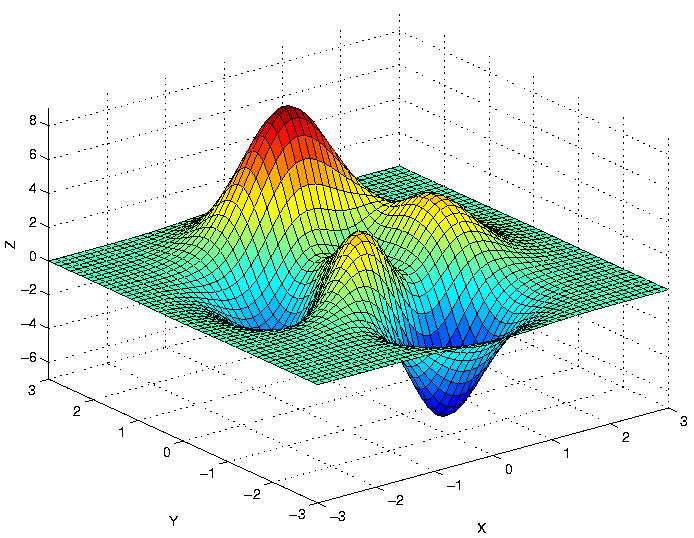
\includegraphics[width=0.45\textwidth]{Images/Gradient.png}
	\caption{\textbf{Multidimensional graph with hills and valleys.}}
\end{wrapfigure}
We can picture this visually by observing figure 2 to the right. Imagine that we have a ball at rest anywhere in this graph with a goal of reaching the lowest point in the graph. We start by finding the gradient of the spot that the ball is currently at. From this, we can determine which way is down and we also have a slope at the current point. Using both of these together we can both move down toward a lower point and at the same time we can move the ball a distance in proportion to the slope that it is currently at. As the ball gets closer to a minimum point, the slope gets smaller so the ball in turn moves slower as well. By the time the ball gets to the lowest point, it is moving very slowly. The error function previously shown allows us to determine how fast the ball should move and where it should move based on the accumulated costs of the network. The version of gradient descent used in this implementation is called Stochastic Gradient Descent and it uses small batches of around 15 inputs \--- which we refer to as mini-batches \--- in order to improve calculation time as this process would use a lot of memory to store everything if done in one large batch. Now that we've calculated our gradient and errors, the next step is to send these values back through the network to update the previous layer's nodes and their activations and weights.

\subsection{Backward Propagation}
The last element of our neural network is backward propagation which as previously stated is the act of sending errors calculated at the output layer back through the network to update weights and activations along the way.

\section{Implementation}

\section{Experiments and Results}

\section{Applications}

\section{Conclusion}

\section*{References}


\end{document}

% Wrapfig example
\begin{wrapfigure}{r}{0.5\textwidth}
	\centering
	\includegraphics[width=0.35\textwidth]{FFNN.jpg}
\end{wrapfigure}

% Algorithm Block Example
\begin{algorithm}
    \SetKwInOut{Input}{Input}
    \SetKwInOut{Output}{Output}

    \underline{function Euclid} $(a,b)$\;
    \Input{Two nonnegative integers $a$ and $b$}
    \Output{$\gcd(a,b)$}
    \eIf{$b=0$}
      {
        return $a$\;
      }
      {
        return Euclid$(b,a\mod b)$\;
      }
    \caption{Euclid's algorithm for finding the greatest common divisor of two nonnegative integers}
\end{algorithm}